% !TEX encoding = UTF-8 Unicode
%!TEX root = main.tex
% !TEX spellcheck = en-US
%%=========================================

%%%%%%%%%%%%%%%%%%%%%%%%%%%%%%%%%%%%%%%%%%%%%%%%%%%%%%%%%%%%%%%%%%%%%%%%%%%%%%%%
\chapter{Performance}
\label{ch:performance}

Benchmarking performance of a concurrency library is difficult. Some might even argue performance is not important, but rather the abstractions are correct. However, some metrics and parallel design patterns can be tested. 

The idea is to create some concurrent programs with different degrees of parallelism. Metrics such as concurrent throughput, sequential speed, and load balancing are factors which can influence performance.

To have some appropriately comparable benchmarks, the library C++CSP and the programming language Go have been chosen because of their dynamic multithreading capabilities. To show the direct increase with multicore utilization, the singlecore equivalent test implementations of ProXC++ and Go are also included. C++CSP does not have any facilities to limit the resource utilization to singlecore, and therefore only have the multicore implementations included.

The libraries Cilk/CilkPlus and C++CSP2 would have been perfect entries for this benchmark. However, because of proprietary software licenses with Cilk and major difficulties getting C++CSP2 programs to work properly, the libraries was left out.

FIXME should not be the only metric


%%%%%%%%%%%%%%%%%%%%%%%%%%%%%%%%%%%%%%%%%%%%%%%%%%%%%%%%%%%%%%%%%%%%%%%%%%%%%%%%
\section{Benchmark Setup}
\label{sec:benchmark_setup}

All benchmarks performed in this chapter are computed on the same machine; a desktop PC with an Intel\textregistered{} Core\texttrademark{} i7-4790 4GHz processor with 8 logical cores, 16GiB DDR3 RAM, running Ubuntu\textregistered{} 16.04 xenial, x86\_64 Linux\textregistered{} 4.4.0 as operating system.

Intel Core is a registered trademark of Intel Corporation, Linux is the registered trademark of Linus Torvaldsen in the U.S. and other countries, Ubuntu is a registered trademark of Canonical Ltd.


%%%%%%%%%%%%%%%%%%%%%%%%%%%%%%%%%%%%%%%%%%%%%%%%%%%%%%%%%%%%%%%%%%%%%%%%%%%%%%%%
\section{Benchmark Tests}
\label{sec:benchmark_tests}


Three type of benchmark tests are performed: \textit{extended commstime}, \textit{concurrent mandelbrot} and \textit{concurrent prime sieve}. These three tests have various degrees of sequential and parallel characteristics, aiming to highlight the concurrency adaptation capabilities and concurrent throughput of each entry.


%%%%%%%%%%%%%%%%%%%%%%%%%%%%%%%%%%%%%%%%
\subsection{Extended Commstime}


The extended commstime test is a custom derivation of the original commstime test. The original commstime test \citep{roger2001commstime} is a pseudo\hyp{}standard benchmark for test sequential channel communication between processes. Three processes called \textit{prefix}, \textit{delta} and \textit{successor} creates a channel cycle, sending an integer in loops. Each loop increments the integer. A fourth process called \textit{consumer} receives the integer on each loop cycle. The consumer receives a number of integers and calculates the average time to receive the integer. The commstime test mostly gives a metric for the overhead regarding channel communication.

Channel communication overhead is not that interesting of a metric with dynamic multithreading. Commstime is however a good metric for a programs adaptability of sequential programs. I therefore propose the \textit{extended commstime} test. Instead of three processes in a channel communication cycle, $N$ processes are created in a chain of channel communications, creating a variable sized cycle.

The extended commstime varies the chain length from $N=1$ to $1000$. Each chain with a given $N$ calculates the average time to receive $100$ integer over $50$ runs. The results are presented in 

\begin{figure}[h!]
    \centering
    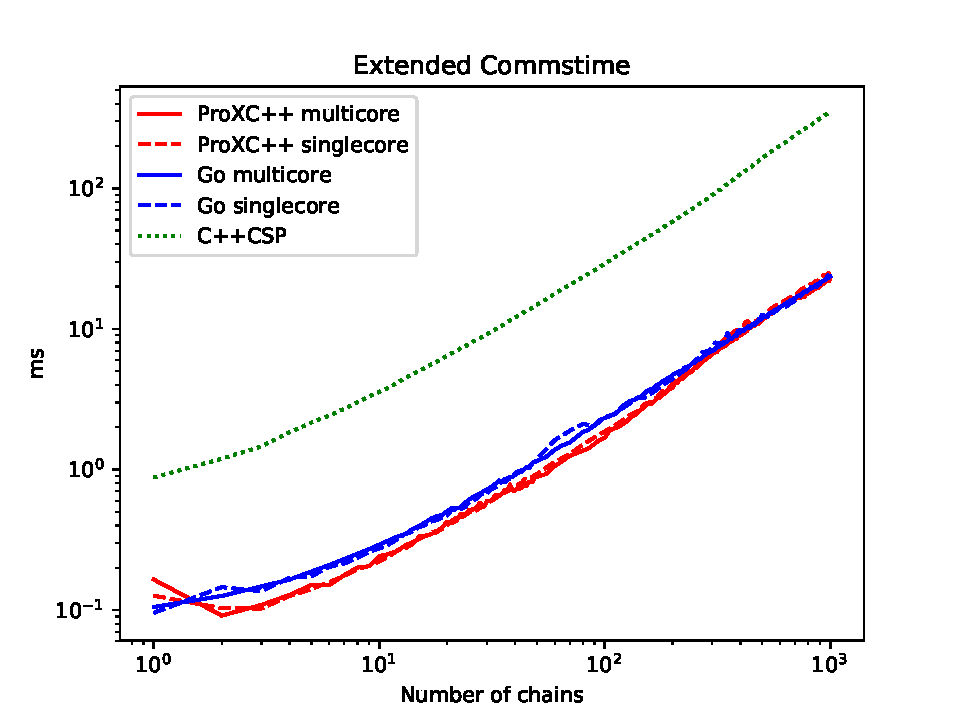
\includegraphics[width=0.8\linewidth]{fig/extended_commstime}
    \caption{Results of extended commstime.}
    \label{fig:extended_commstime}
\end{figure}


%%%%%%%%%%%%%%%%%%%%%%%%%%%%%%%%%%%%%%%%
\subsection{Concurrent Mandelbrot}


Some problems are embarrassingly parallel \citep{wilkinson1999parallel}, where little to no effort is needed to separate the work load into parallel tasks. The mandelbrot set is a perfect example of an embarrassingly parallel problem, where each point in the set can be calculated independently of each other.

Generating a mandelbrot set is perfect for testing the parallel capabilities of the entries, as well as how good the load balancing is.

The mandelbrot set of a given dimension is computed in a map\hyp{}reduce manner, where a number of workers are working in parallel and their results are collected by a single consumer. Each worker computes a column of the set. Two versions of the map\hyp{}reduce is tested: one where the number of workers are fixed to the number of available cores, and one where one worker is spawned for each column. The idea is to first test the optimal setup of workers, while the second tests the load balancing capabilities of the entries. 

\begin{figure}[h!]
    \centering
    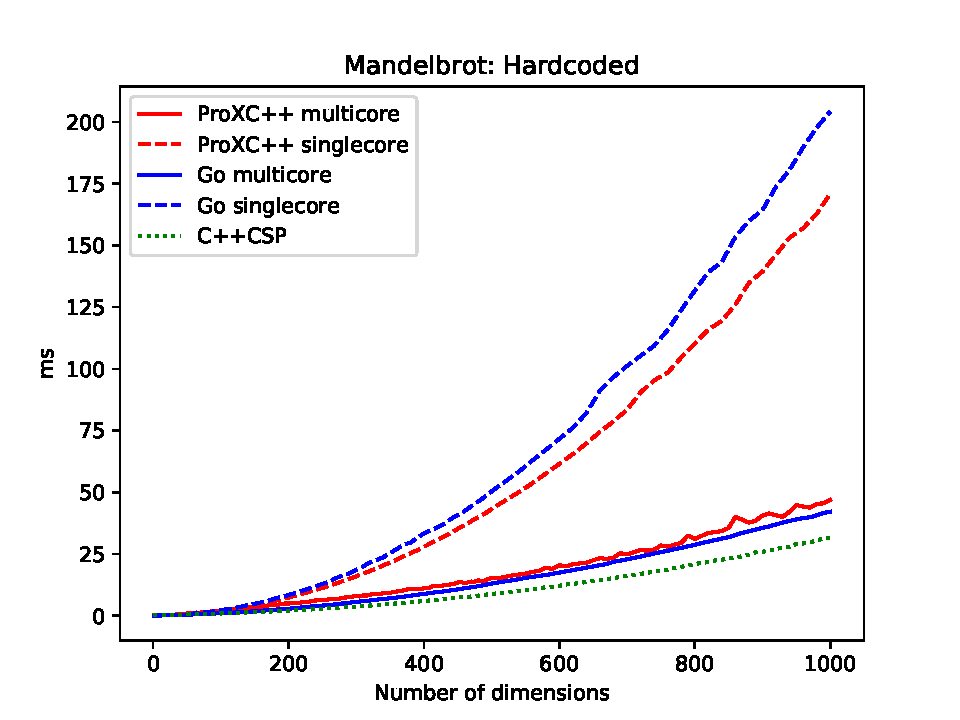
\includegraphics[width=0.8\linewidth]{fig/mandelbrot_hardcoded}
    \caption{Results of concurrent mandelbrot with hardcoded number of workers.}
    \label{fig:mandelbrot_hardcoded}
\end{figure}

\begin{figure}[h!]
    \centering
    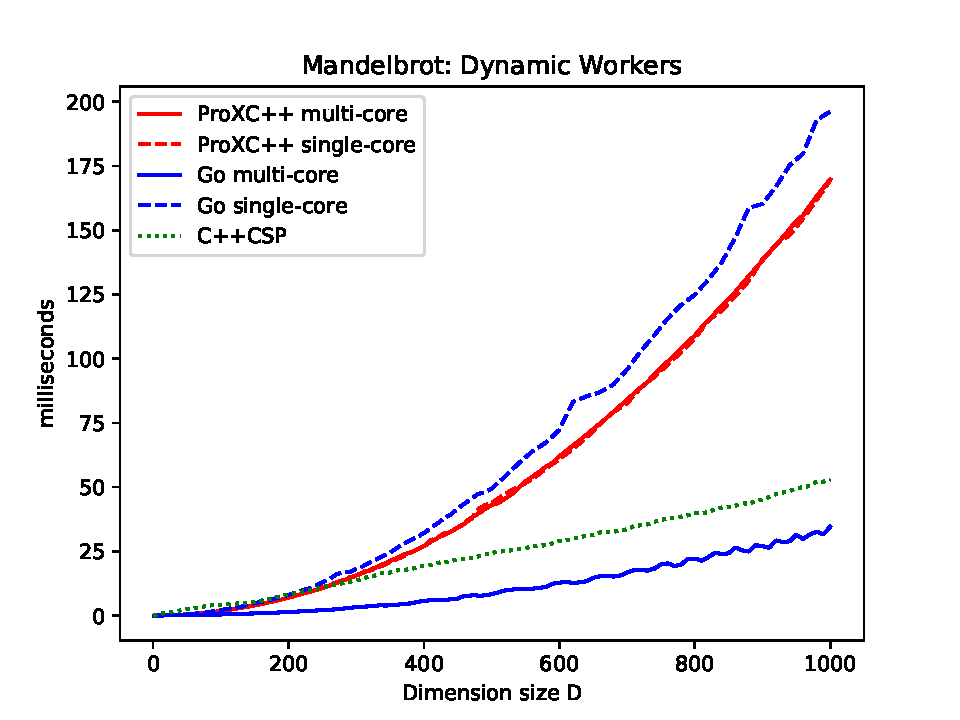
\includegraphics[width=0.8\linewidth]{fig/mandelbrot_dynamic}
    \caption{Results of concurrent mandelbrot with dynamic number of workers.}
    \label{fig:mandelbrot_dynamic}
\end{figure}


%%%%%%%%%%%%%%%%%%%%%%%%%%%%%%%%%%%%%%%%
\subsection{Concurrent Prime Sieve}


The last benchmark is the concurrent prime sieve, popularized by the famously elegant piece of concurrent code in Go \citep{go2017primesieve}. A prime sieve is a fast type of algorithm to find prime numbers, usually implemented as a sequential algorithm. A concurrent prime sieve is also an algorithm to find prime numbers, however daisy\hyp{}chains processes to determine whether a number is a prime or not.

At the start of the daisy\hyp{}chain is the \textit{generator}, which generates all numbers from $2$ and above. Along the daisy\hyp{}chain is \textit{filters}, where each filters represent a prime number along the number line. When the filter receives a number the divisibility is checked. A non\hyp{}divisible number is passed along the daisy\hyp{}chain, while a divisible number is discarded. Given a daisy\hyp{}chain of $N$ filters, at the end is the $N$th prime.

This benchmark tests generating $N$ prime numbers, where $N=10$ to $1000$. Given a $N$, the execution time per prime number is calculated over the average running time of $10$ runs.

\begin{figure}[h!]
    \centering
    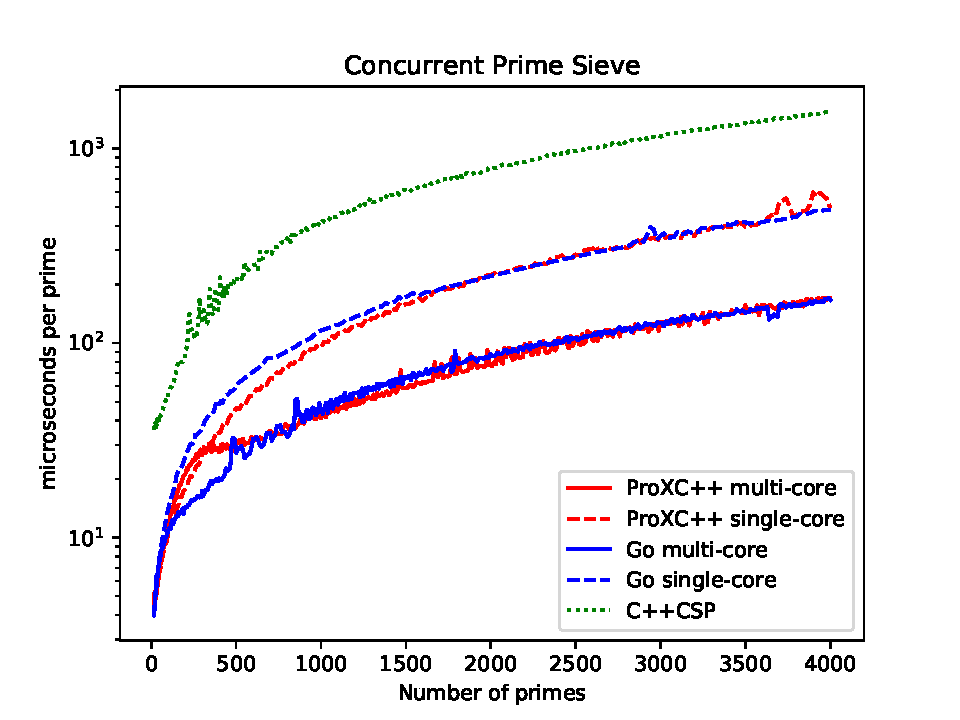
\includegraphics[width=0.8\linewidth]{fig/concurrent_sieve}
    \caption{Results of concurrent sieve.}
    \label{fig:concurrent_sieve}
\end{figure}


%%%%%%%%%%%%%%%%%%%%%%%%%%%%%%%%%%%%%%%%%%%%%%%%%%%%%%%%%%%%%%%%%%%%%%%%%%%%%%%%
\section{Analysis}
\label{sec:analysis}


